\documentclass[11pt,a4paper]{article}
\usepackage[margin=1in]{geometry}
\usepackage{amsmath,amssymb,amsthm}
\usepackage{mathtools}
\usepackage{enumitem}
\usepackage{xcolor}
\usepackage{tikz}
\usetikzlibrary{arrows.meta,decorations.markings}

% Custom commands for XYZ methodology
\newcommand{\stage}[1]{\textbf{\textcolor{blue}{#1}}}
\newcommand{\critical}[1]{\textbf{\textcolor{red}{#1}}}

\title{Exercise Sheet 1, Question 5: 2D Phase Portraits\\
Complete Solution with XYZ Methodology\\
Methods of Applied Mathematics [SEMT30006]}
\author{}
\date{}

\begin{document}

\maketitle

\section*{Problem Statement}

Sketch phase portraits for the following differential equations and classify the equilibria.

\begin{enumerate}[label=(\alph*)]
    \item $\frac{du}{dt} = v^2 - u$, $\frac{dv}{dt} = u^2 - v$
    \item $\frac{d^2u}{dt^2} + \frac{du}{dt} + \sin(u) = 0$
\end{enumerate}

\section{Foundational Concepts: 2D Phase Portraits}

\subsection*{What is a 2D Phase Portrait?}

\begin{itemize}[leftmargin=*]
\item \stage{STAGE X (Definition):}
For a 2D autonomous system:
\begin{align}
\frac{du}{dt} = f(u, v), \quad \frac{dv}{dt} = g(u, v)
\end{align}

The \textbf{phase portrait} is a visualization in the $(u, v)$ plane showing:
\begin{itemize}
    \item \textbf{Equilibria} (fixed points): where $f = 0$ and $g = 0$
    \item \textbf{Nullclines}: curves where $\dot{u} = 0$ or $\dot{v} = 0$
    \item \textbf{Vector field}: arrows $(f, g)$ showing direction of flow
    \item \textbf{Trajectories}: solution curves $(u(t), v(t))$ in the plane
\end{itemize}

\item \stage{STAGE Y (Key tools for analysis):}
\begin{enumerate}
    \item \textbf{Nullclines}:
    \begin{itemize}
        \item $u$-nullcline: where $\dot{u} = 0$ (flow vertical)
        \item $v$-nullcline: where $\dot{v} = 0$ (flow horizontal)
        \item Equilibria: intersections of nullclines
    \end{itemize}
    \item \textbf{Linearization}: Near equilibrium $(u^*, v^*)$, approximate:
    \begin{align}
    \begin{pmatrix} \dot{u} \\ \dot{v} \end{pmatrix} \approx J \begin{pmatrix} u - u^* \\ v - v^* \end{pmatrix}
    \end{align}
    where $J$ is the Jacobian matrix.
    \item \textbf{Eigenvalues of $J$}: Determine local behavior
\end{enumerate}

\item \stage{STAGE Z (Classification by eigenvalues):}
For Jacobian with eigenvalues $\lambda_1, \lambda_2$:
\begin{itemize}
    \item \textbf{Node} (both $\lambda$ real, same sign):
    \begin{itemize}
        \item Stable if $\lambda_1, \lambda_2 < 0$
        \item Unstable if $\lambda_1, \lambda_2 > 0$
    \end{itemize}
    \item \textbf{Saddle} (both $\lambda$ real, opposite signs): Always unstable
    \item \textbf{Focus/Spiral} ($\lambda = \alpha \pm i\beta$, complex conjugates):
    \begin{itemize}
        \item Stable if $\alpha < 0$
        \item Unstable if $\alpha > 0$
    \end{itemize}
    \item \textbf{Center} ($\lambda = \pm i\beta$, purely imaginary): Neutrally stable
\end{itemize}
\end{itemize}

\critical{FROM LECTURE NOTES (pages 29-34):} The trace and determinant of the Jacobian determine equilibrium type:
\begin{align}
\tau = \text{tr}(J) = \lambda_1 + \lambda_2, \quad \Delta = \det(J) = \lambda_1 \lambda_2
\end{align}

\newpage

\section{Part (a): $\frac{du}{dt} = v^2 - u$, $\frac{dv}{dt} = u^2 - v$}

\subsection*{Step 1: Identify System Structure and Symmetry}

\begin{itemize}[leftmargin=*]
\item \stage{STAGE X (System form):}
\begin{align}
\dot{u} &= v^2 - u = f(u, v) \\
\dot{v} &= u^2 - v = g(u, v)
\end{align}

This is a coupled nonlinear system with quadratic terms.

\item \stage{STAGE Y (Symmetry observation):}
The system has a beautiful symmetry: swapping $u \leftrightarrow v$ leaves the system unchanged!

If $(u(t), v(t))$ is a solution, then $(v(t), u(t))$ is also a solution.

This means:
\begin{itemize}
    \item Phase portrait is symmetric about the line $v = u$
    \item If $(a, b)$ is an equilibrium, so is $(b, a)$
    \item Trajectories are mirror images across $v = u$
\end{itemize}

\item \stage{STAGE Z (Implications):}
We can exploit this symmetry when:
\begin{itemize}
    \item Finding equilibria
    \item Sketching phase portraits
    \item Understanding global dynamics
\end{itemize}
\end{itemize}

\subsection*{Step 2: Find Equilibria}

\begin{itemize}[leftmargin=*]
\item \stage{STAGE X (Equilibrium conditions):}
At equilibrium: $\dot{u} = 0$ and $\dot{v} = 0$:
\begin{align}
v^2 - u &= 0 \quad \Rightarrow \quad u = v^2 \\
u^2 - v &= 0 \quad \Rightarrow \quad v = u^2
\end{align}

\item \stage{STAGE Y (Solving the system):}
Substitute $u = v^2$ into $v = u^2$:
\begin{align}
v = (v^2)^2 = v^4
\end{align}

Rearranging:
\begin{align}
v^4 - v = 0 \quad \Rightarrow \quad v(v^3 - 1) = 0
\end{align}

So $v = 0$ or $v^3 = 1$.

For $v^3 = 1$: only real solution is $v = 1$.

Therefore: $v \in \{0, 1\}$

For each $v$, find corresponding $u$:
\begin{itemize}
    \item If $v = 0$: $u = v^2 = 0$ $\Rightarrow$ equilibrium at $(0, 0)$
    \item If $v = 1$: $u = v^2 = 1$ $\Rightarrow$ equilibrium at $(1, 1)$
\end{itemize}

\item \stage{STAGE Z (Two equilibria):}
\begin{align}
\boxed{(u^*, v^*) = (0, 0) \text{ and } (1, 1)}
\end{align}

Note: Both lie on the symmetry line $v = u$ (as expected from symmetry).
\end{itemize}

\subsection*{Step 3: Find and Sketch Nullclines}

\begin{itemize}[leftmargin=*]
\item \stage{STAGE X ($u$-nullcline):}
Where $\dot{u} = 0$:
\begin{align}
v^2 - u = 0 \quad \Rightarrow \quad u = v^2
\end{align}

This is a parabola opening to the right. On this curve, flow is purely vertical.

\item \stage{STAGE Y ($v$-nullcline):}
Where $\dot{v} = 0$:
\begin{align}
u^2 - v = 0 \quad \Rightarrow \quad v = u^2
\end{align}

This is a parabola opening upward. On this curve, flow is purely horizontal.

\item \stage{STAGE Z (Intersections):}
The nullclines intersect where both $u = v^2$ and $v = u^2$, which gives our equilibria $(0,0)$ and $(1,1)$ as found above.

The nullclines divide the plane into regions with different flow directions.
\end{itemize}

\subsection*{Step 4: Determine Flow Direction in Each Region}

\begin{itemize}[leftmargin=*]
\item \stage{STAGE X (Sign analysis):}
The nullclines divide the $(u,v)$ plane into several regions. We determine the sign of $\dot{u}$ and $\dot{v}$ in each:

\begin{itemize}
    \item $\dot{u} = v^2 - u > 0$ when $u < v^2$ (left of $u$-nullcline)
    \item $\dot{u} = v^2 - u < 0$ when $u > v^2$ (right of $u$-nullcline)
    \item $\dot{v} = u^2 - v > 0$ when $v < u^2$ (below $v$-nullcline)
    \item $\dot{v} = u^2 - v < 0$ when $v > u^2$ (above $v$-nullcline)
\end{itemize}

\item \stage{STAGE Y (Test points):}

\textbf{Region between parabolas (e.g., point $(0.5, 0.5)$):}
\begin{align}
\dot{u} = (0.5)^2 - 0.5 = -0.25 < 0 \quad &\Rightarrow \quad \text{flow LEFT} \\
\dot{v} = (0.5)^2 - 0.5 = -0.25 < 0 \quad &\Rightarrow \quad \text{flow DOWN}
\end{align}
Flow is $\searrow$ (southwest)

\textbf{Region below both parabolas (e.g., point $(2, 0.5)$):}
\begin{align}
\dot{u} = (0.5)^2 - 2 = -1.75 < 0 \quad &\Rightarrow \quad \text{flow LEFT} \\
\dot{v} = (2)^2 - 0.5 = 3.5 > 0 \quad &\Rightarrow \quad \text{flow UP}
\end{align}
Flow is $\nwarrow$ (northwest)

\textbf{Region above both parabolas (e.g., point $(0.5, 2)$):}
\begin{align}
\dot{u} = (2)^2 - 0.5 = 3.5 > 0 \quad &\Rightarrow \quad \text{flow RIGHT} \\
\dot{v} = (0.5)^2 - 2 = -1.75 < 0 \quad &\Rightarrow \quad \text{flow DOWN}
\end{align}
Flow is $\searrow$ (southeast)

\item \stage{STAGE Z (Flow pattern):}
The flow patterns suggest spiral or rotational behavior around equilibria, with the parabolas guiding the flow.
\end{itemize}

\subsection*{Step 5: Linearization at $(0, 0)$}

\begin{itemize}[leftmargin=*]
\item \stage{STAGE X (Compute Jacobian):}
The Jacobian matrix is:
\begin{align}
J = \begin{pmatrix}
\frac{\partial f}{\partial u} & \frac{\partial f}{\partial v} \\
\frac{\partial g}{\partial u} & \frac{\partial g}{\partial v}
\end{pmatrix}
= \begin{pmatrix}
-1 & 2v \\
2u & -1
\end{pmatrix}
\end{align}

At $(u^*, v^*) = (0, 0)$:
\begin{align}
J(0,0) = \begin{pmatrix}
-1 & 0 \\
0 & -1
\end{pmatrix} = -I
\end{align}

\item \stage{STAGE Y (Find eigenvalues):}
For $J = -I$, the characteristic equation is:
\begin{align}
\det(J - \lambda I) = \det\begin{pmatrix}
-1-\lambda & 0 \\
0 & -1-\lambda
\end{pmatrix} = (-1-\lambda)^2 = 0
\end{align}

Therefore:
\begin{align}
\lambda_1 = \lambda_2 = -1
\end{align}

Both eigenvalues are real, negative, and equal (repeated eigenvalue).

\item \stage{STAGE Z (Classification):}
\begin{align}
\boxed{\text{Stable node (star node)}}
\end{align}

Since $J = -I$:
\begin{itemize}
    \item All directions are eigendirections
    \item Trajectories approach origin along straight lines
    \item This is called a \textbf{star node} or \textbf{proper node}
    \item Decay rate: $e^{-t}$ (time constant $\tau = 1$)
\end{itemize}
\end{itemize}

\subsection*{Step 6: Linearization at $(1, 1)$}

\begin{itemize}[leftmargin=*]
\item \stage{STAGE X (Jacobian at $(1,1)$):}
\begin{align}
J(1,1) = \begin{pmatrix}
-1 & 2(1) \\
2(1) & -1
\end{pmatrix}
= \begin{pmatrix}
-1 & 2 \\
2 & -1
\end{pmatrix}
\end{align}

\item \stage{STAGE Y (Find eigenvalues):}
Characteristic equation:
\begin{align}
\det(J - \lambda I) = \det\begin{pmatrix}
-1-\lambda & 2 \\
2 & -1-\lambda
\end{pmatrix} = 0
\end{align}

\begin{align}
(-1-\lambda)^2 - 4 &= 0 \\
\lambda^2 + 2\lambda + 1 - 4 &= 0 \\
\lambda^2 + 2\lambda - 3 &= 0 \\
(\lambda + 3)(\lambda - 1) &= 0
\end{align}

Therefore:
\begin{align}
\lambda_1 = -3, \quad \lambda_2 = +1
\end{align}

One negative, one positive (opposite signs).

\item \stage{STAGE Z (Classification):}
\begin{align}
\boxed{\text{Saddle point (unstable)}}
\end{align}

Since eigenvalues have opposite signs:
\begin{itemize}
    \item One stable direction (along eigenvector for $\lambda_1 = -3$)
    \item One unstable direction (along eigenvector for $\lambda_2 = +1$)
    \item Saddle points are always unstable (hyperbolic)
    \item $\det(J) = \lambda_1 \lambda_2 = -3 < 0$ confirms saddle
\end{itemize}
\end{itemize}

\subsection*{Step 7: Find Eigenvectors for Saddle at $(1,1)$}

\begin{itemize}[leftmargin=*]
\item \stage{STAGE X (Eigenvector for $\lambda_1 = -3$):}
Solve $(J - \lambda_1 I)\mathbf{v}_1 = 0$:
\begin{align}
\begin{pmatrix}
-1-(-3) & 2 \\
2 & -1-(-3)
\end{pmatrix}\begin{pmatrix} v_1 \\ v_2 \end{pmatrix}
= \begin{pmatrix}
2 & 2 \\
2 & 2
\end{pmatrix}\begin{pmatrix} v_1 \\ v_2 \end{pmatrix}
= \mathbf{0}
\end{align}

From first row: $2v_1 + 2v_2 = 0$ $\Rightarrow$ $v_1 = -v_2$

Eigenvector: $\mathbf{v}_1 = \begin{pmatrix} 1 \\ -1 \end{pmatrix}$

\textbf{Stable manifold:} Along direction $(1, -1)$ from $(1,1)$

\item \stage{STAGE Y (Eigenvector for $\lambda_2 = +1$):}
Solve $(J - \lambda_2 I)\mathbf{v}_2 = 0$:
\begin{align}
\begin{pmatrix}
-1-1 & 2 \\
2 & -1-1
\end{pmatrix}\begin{pmatrix} v_1 \\ v_2 \end{pmatrix}
= \begin{pmatrix}
-2 & 2 \\
2 & -2
\end{pmatrix}\begin{pmatrix} v_1 \\ v_2 \end{pmatrix}
= \mathbf{0}
\end{align}

From first row: $-2v_1 + 2v_2 = 0$ $\Rightarrow$ $v_1 = v_2$

Eigenvector: $\mathbf{v}_2 = \begin{pmatrix} 1 \\ 1 \end{pmatrix}$

\textbf{Unstable manifold:} Along direction $(1, 1)$ from $(1,1)$

\item \stage{STAGE Z (Geometric interpretation):}
At the saddle point $(1,1)$:
\begin{itemize}
    \item Stable direction: slope $-1$ (line through origin and $(1,1)$ with negative slope)
    \item Unstable direction: slope $+1$ (the symmetry line $v = u$)
    \item Trajectories approach along stable manifold, repel along unstable manifold
\end{itemize}

Note: The unstable direction lies exactly on the symmetry line $v = u$!
\end{itemize}

\subsection*{Step 8: Sketch Phase Portrait}

\begin{itemize}[leftmargin=*]
\item \stage{STAGE X (Key features to include):}
\begin{enumerate}
    \item Both nullclines (parabolas)
    \item Two equilibria with classifications
    \item Eigendirections at saddle
    \item Flow directions in each region
    \item Representative trajectories
    \item Symmetry about $v = u$
\end{enumerate}

\item \stage{STAGE Y (Phase portrait):}

\begin{center}
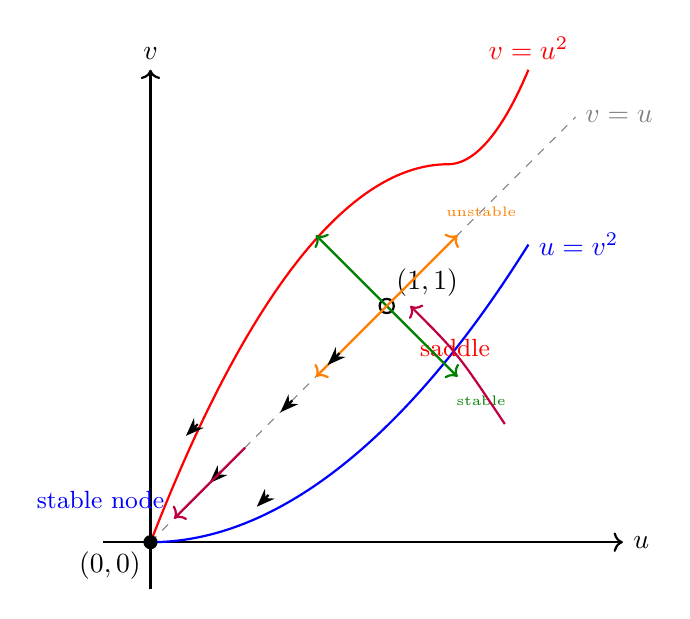
\begin{tikzpicture}[scale=3]
    % Axes
    \draw[->,thick] (-0.2,0) -- (2,0) node[right] {$u$};
    \draw[->,thick] (0,-0.2) -- (0,2) node[above] {$v$};

    % Symmetry line
    \draw[dashed,gray] (0,0) -- (1.8,1.8) node[right] {$v=u$};

    % Nullclines
    \draw[thick,blue] (0,0) parabola (1.6,1.26) node[right] {$u=v^2$};
    \draw[thick,red] (0,0) parabola bend (1.26,1.6) (1.6,2) node[above] {$v=u^2$};

    % Equilibria
    \fill[black] (0,0) circle (0.03);
    \node[below left] at (0,0) {$(0,0)$};
    \node[above left,blue] at (0.1,0.1) {\small stable node};

    \fill[white,draw=black,thick] (1,1) circle (0.03);
    \node[above right] at (1,1) {$(1,1)$};
    \node[below right,red] at (1.1,0.9) {\small saddle};

    % Stable and unstable manifolds at saddle
    \draw[->,thick,green!50!black] (1,1) -- (1.3,0.7);
    \draw[->,thick,green!50!black] (1,1) -- (0.7,1.3);
    \node[green!50!black] at (1.4,0.6) {\tiny stable};

    \draw[->,thick,orange] (1,1) -- (0.7,0.7);
    \draw[->,thick,orange] (1,1) -- (1.3,1.3);
    \node[orange] at (1.4,1.4) {\tiny unstable};

    % Flow arrows in different regions
    % Near origin
    \draw[-{Stealth},thick] (0.3,0.3) -- (0.25,0.25);
    \draw[-{Stealth},thick] (0.5,0.2) -- (0.45,0.15);
    \draw[-{Stealth},thick] (0.2,0.5) -- (0.15,0.45);

    % Between parabolas
    \draw[-{Stealth},thick] (0.6,0.6) -- (0.55,0.55);
    \draw[-{Stealth},thick] (0.8,0.8) -- (0.75,0.75);

    % Sample trajectories
    \draw[->,thick,purple] (0.4,0.4) .. controls (0.3,0.3) .. (0.1,0.1);
    \draw[->,thick,purple] (1.5,0.5) .. controls (1.3,0.8) .. (1.1,1.0);
\end{tikzpicture}
\end{center}

\item \stage{STAGE Z (Description):}
\begin{itemize}
    \item Blue curve: $u$-nullcline $u = v^2$
    \item Red curve: $v$-nullcline $v = u^2$
    \item Black dot at $(0,0)$: stable node
    \item White dot at $(1,1)$: saddle
    \item Green arrows: stable manifold
    \item Orange arrows: unstable manifold
    \item Trajectories spiral into origin
    \item Saddle creates hyperbolic structure at $(1,1)$
\end{itemize}
\end{itemize}

\subsection*{Step 9: Global Dynamics}

\begin{itemize}[leftmargin=*]
\item \stage{STAGE X (Long-time behavior):}
\begin{enumerate}
    \item Most trajectories converge to the stable node at $(0,0)$
    \item The stable manifold of the saddle forms a boundary
    \item Trajectories on the unstable manifold leave $(1,1)$ along $v = u$
    \item System exhibits strong attraction to origin
\end{enumerate}

\item \stage{STAGE Y (Basin of attraction):}
The basin of attraction for $(0,0)$ is most of the positive quadrant, except:
\begin{itemize}
    \item Points exactly on unstable manifold of saddle
    \item These go to infinity along $v = u$ direction
\end{itemize}

\item \stage{STAGE Z (Physical interpretation):}
This could model:
\begin{itemize}
    \item Two coupled populations with quadratic growth terms
    \item Symmetric competition with nonlinear effects
    \item System with inherent damping ($-u$ and $-v$ terms) balanced by growth ($v^2$ and $u^2$)
\end{itemize}

The saddle at $(1,1)$ represents an unstable coexistence state.
\end{itemize}

\critical{KEY INSIGHT:} The symmetry $u \leftrightarrow v$ creates mirror-image dynamics across $v = u$. The saddle's unstable manifold lies exactly on this symmetry line, making it a special separatrix in the system.

\newpage

\section{Part (b): $\frac{d^2u}{dt^2} + \frac{du}{dt} + \sin(u) = 0$}

\subsection*{Step 1: Convert to First-Order System}

\begin{itemize}[leftmargin=*]
\item \stage{STAGE X (Standard procedure):}
This is a second-order ODE. To analyze it in the phase plane, introduce:
\begin{align}
v = \frac{du}{dt}
\end{align}

Then:
\begin{align}
\frac{dv}{dt} = \frac{d^2u}{dt^2}
\end{align}

\item \stage{STAGE Y (Rewrite as system):}
From the original equation:
\begin{align}
\frac{d^2u}{dt^2} = -\frac{du}{dt} - \sin(u) = -v - \sin(u)
\end{align}

Therefore, the first-order system is:
\begin{align}
\frac{du}{dt} &= v \\
\frac{dv}{dt} &= -v - \sin(u)
\end{align}

\item \stage{STAGE Z (Phase space interpretation):}
\begin{itemize}
    \item $(u, v)$ is the phase space (position and velocity)
    \item $u$: displacement (like angle of pendulum)
    \item $v = \dot{u}$: velocity
    \item This represents a damped nonlinear oscillator
\end{itemize}
\end{itemize}

\subsection*{Step 2: Physical Interpretation}

\begin{itemize}[leftmargin=*]
\item \stage{STAGE X (Pendulum analogy):}
The equation $\ddot{u} + \dot{u} + \sin(u) = 0$ models a damped pendulum:
\begin{itemize}
    \item $\sin(u)$: restoring force (gravity)
    \item $\dot{u}$: damping (friction)
    \item $\ddot{u}$: acceleration
\end{itemize}

For small angles: $\sin(u) \approx u$, recovering the simple harmonic oscillator with damping.

\item \stage{STAGE Y (Energy consideration):}
This system is dissipative (loses energy due to damping term $\dot{u}$). We expect:
\begin{itemize}
    \item No closed orbits (energy decreases)
    \item Convergence to equilibria
    \item No periodic solutions
\end{itemize}

\item \stage{STAGE Z (Periodicity in $u$):}
Since $\sin(u)$ is periodic with period $2\pi$:
\begin{itemize}
    \item Phase portrait repeats every $2\pi$ in the $u$-direction
    \item Equilibria at $u = n\pi$ for integer $n$
    \item We typically plot one or two periods: $u \in [-\pi, 3\pi]$
\end{itemize}
\end{itemize}

\subsection*{Step 3: Find Equilibria}

\begin{itemize}[leftmargin=*]
\item \stage{STAGE X (Equilibrium conditions):}
At equilibrium:
\begin{align}
\dot{u} = v &= 0 \\
\dot{v} = -v - \sin(u) &= 0
\end{align}

From first equation: $v = 0$

From second equation: $-0 - \sin(u) = 0$ $\Rightarrow$ $\sin(u) = 0$

\item \stage{STAGE Y (Solving):}
$\sin(u) = 0$ when $u = n\pi$ for any integer $n$.

Therefore:
\begin{align}
\text{Equilibria: } (u^*, v^*) = (n\pi, 0) \text{ for } n \in \mathbb{Z}
\end{align}

\item \stage{STAGE Z (Infinite equilibria):}
\begin{align}
\ldots, (-2\pi, 0), (-\pi, 0), (0, 0), (\pi, 0), (2\pi, 0), (3\pi, 0), \ldots
\end{align}

For analysis, we focus on:
\begin{itemize}
    \item $(0, 0)$: corresponds to pendulum hanging down (stable)
    \item $(\pi, 0)$: corresponds to pendulum pointing up (unstable)
    \item Pattern repeats every $2\pi$
\end{itemize}
\end{itemize}

\subsection*{Step 4: Find Nullclines}

\begin{itemize}[leftmargin=*]
\item \stage{STAGE X ($u$-nullcline):}
Where $\dot{u} = 0$:
\begin{align}
v = 0
\end{align}

This is the entire $u$-axis (horizontal line through $v = 0$).

\item \stage{STAGE Y ($v$-nullcline):}
Where $\dot{v} = 0$:
\begin{align}
-v - \sin(u) = 0 \quad \Rightarrow \quad v = -\sin(u)
\end{align}

This is a sinusoidal curve.

\item \stage{STAGE Z (Intersections):}
Nullclines intersect where $v = 0$ and $v = -\sin(u)$:
\begin{align}
0 = -\sin(u) \quad \Rightarrow \quad \sin(u) = 0 \quad \Rightarrow \quad u = n\pi
\end{align}

Confirming our equilibria at $(n\pi, 0)$.
\end{itemize}

\subsection*{Step 5: Linearization and Classification}

\begin{itemize}[leftmargin=*]
\item \stage{STAGE X (Jacobian):}
For the system:
\begin{align}
\dot{u} = v, \quad \dot{v} = -v - \sin(u)
\end{align}

The Jacobian is:
\begin{align}
J = \begin{pmatrix}
0 & 1 \\
-\cos(u) & -1
\end{pmatrix}
\end{align}

\item \stage{STAGE Y (At equilibria $u = n\pi$):}

At even multiples: $u = 0, \pm 2\pi, \pm 4\pi, \ldots$
\begin{align}
J(2n\pi, 0) = \begin{pmatrix}
0 & 1 \\
-\cos(2n\pi) & -1
\end{pmatrix}
= \begin{pmatrix}
0 & 1 \\
-1 & -1
\end{pmatrix}
\end{align}

At odd multiples: $u = \pm \pi, \pm 3\pi, \ldots$
\begin{align}
J((2n+1)\pi, 0) = \begin{pmatrix}
0 & 1 \\
-\cos((2n+1)\pi) & -1
\end{pmatrix}
= \begin{pmatrix}
0 & 1 \\
+1 & -1
\end{pmatrix}
\end{align}

\item \stage{STAGE Z (Two distinct types):}
We need to analyze eigenvalues for each type.
\end{itemize}

\subsection*{Step 6: Classify Equilibria at $u = 2n\pi$ (e.g., $(0,0)$)}

\begin{itemize}[leftmargin=*]
\item \stage{STAGE X (Eigenvalues):}
For $J = \begin{pmatrix} 0 & 1 \\ -1 & -1 \end{pmatrix}$:

Characteristic equation:
\begin{align}
\det(J - \lambda I) = \det\begin{pmatrix}
-\lambda & 1 \\
-1 & -1-\lambda
\end{pmatrix} = \lambda(\lambda + 1) + 1 = 0
\end{align}

\begin{align}
\lambda^2 + \lambda + 1 = 0
\end{align}

Using quadratic formula:
\begin{align}
\lambda = \frac{-1 \pm \sqrt{1 - 4}}{2} = \frac{-1 \pm \sqrt{-3}}{2} = \frac{-1 \pm i\sqrt{3}}{2}
\end{align}

\item \stage{STAGE Y (Complex eigenvalues):}
\begin{align}
\lambda = -\frac{1}{2} \pm i\frac{\sqrt{3}}{2}
\end{align}

These are complex conjugates with:
\begin{itemize}
    \item Real part: $\alpha = -\frac{1}{2} < 0$ (stable)
    \item Imaginary part: $\beta = \pm\frac{\sqrt{3}}{2}$ (oscillations)
\end{itemize}

\item \stage{STAGE Z (Classification):}
\begin{align}
\boxed{\text{Stable focus (spiral sink)}}
\end{align}

Equilibria at $(0, 0), (\pm 2\pi, 0), (\pm 4\pi, 0), \ldots$ are stable spirals.

Physical meaning: pendulum hanging down—stable equilibrium with damped oscillations.
\end{itemize}

\subsection*{Step 7: Classify Equilibria at $u = (2n+1)\pi$ (e.g., $(\pi, 0)$)}

\begin{itemize}[leftmargin=*]
\item \stage{STAGE X (Eigenvalues):}
For $J = \begin{pmatrix} 0 & 1 \\ 1 & -1 \end{pmatrix}$:

Characteristic equation:
\begin{align}
\det(J - \lambda I) = \det\begin{pmatrix}
-\lambda & 1 \\
1 & -1-\lambda
\end{pmatrix} = \lambda(\lambda + 1) - 1 = 0
\end{align}

\begin{align}
\lambda^2 + \lambda - 1 = 0
\end{align}

Using quadratic formula:
\begin{align}
\lambda = \frac{-1 \pm \sqrt{1 + 4}}{2} = \frac{-1 \pm \sqrt{5}}{2}
\end{align}

\item \stage{STAGE Y (Real eigenvalues):}
\begin{align}
\lambda_1 = \frac{-1 - \sqrt{5}}{2} \approx -1.618 < 0 \\
\lambda_2 = \frac{-1 + \sqrt{5}}{2} \approx +0.618 > 0
\end{align}

One negative, one positive (opposite signs).

\item \stage{STAGE Z (Classification):}
\begin{align}
\boxed{\text{Saddle point (unstable)}}
\end{align}

Equilibria at $(\pi, 0), (\pm 3\pi, 0), (\pm 5\pi, 0), \ldots$ are saddles.

Physical meaning: pendulum pointing up—unstable equilibrium (toppling point).
\end{itemize}

\subsection*{Step 8: Sketch Phase Portrait}

\begin{itemize}[leftmargin=*]
\item \stage{STAGE X (Key features):}
\begin{enumerate}
    \item Stable foci at $u = 0, \pm 2\pi, \ldots$
    \item Saddles at $u = \pm \pi, \pm 3\pi, \ldots$
    \item $u$-nullcline: $v = 0$ (horizontal axis)
    \item $v$-nullcline: $v = -\sin(u)$ (sine curve)
    \item Heteroclinic connections between saddles
\end{enumerate}

\item \stage{STAGE Y (Phase portrait):}

\begin{center}
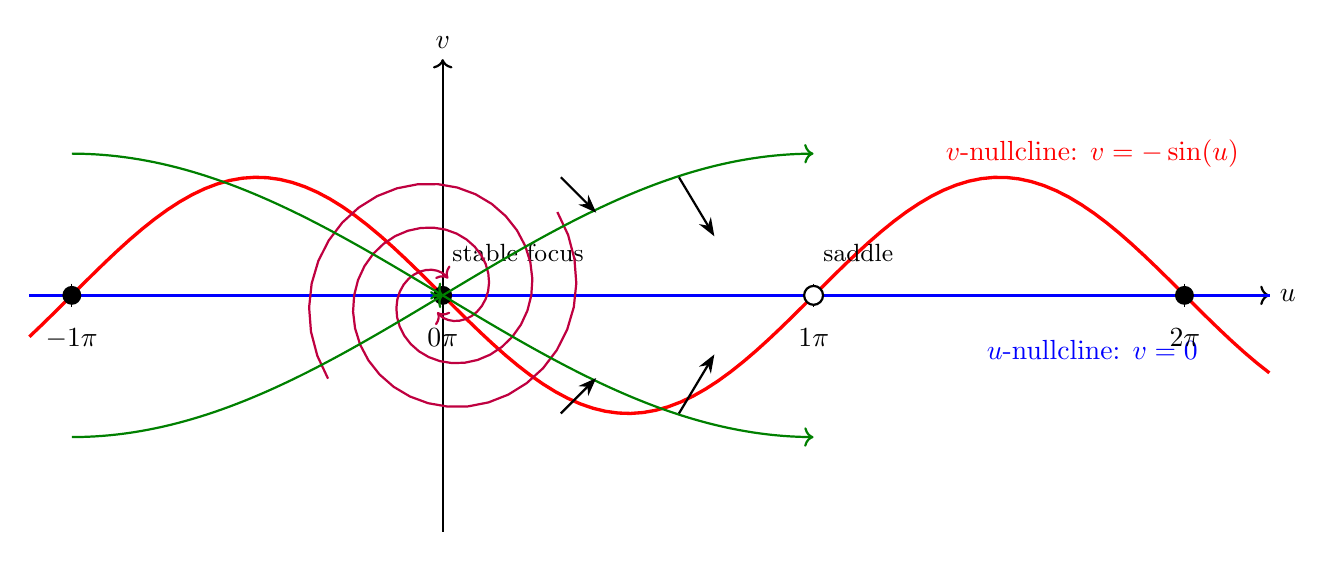
\begin{tikzpicture}[scale=1.5]
    % Axes
    \draw[->,thick] (-3.5,0) -- (7,0) node[right] {$u$};
    \draw[->,thick] (0,-2) -- (0,2) node[above] {$v$};

    % u-nullcline (v = 0)
    \draw[very thick,blue] (-3.5,0) -- (7,0);
    \node[blue,below] at (5.5,-0.3) {$u$-nullcline: $v=0$};

    % v-nullcline (v = -sin(u))
    \draw[very thick,red,domain=-3.5:7,samples=100] plot (\x,{-sin(\x r)});
    \node[red,above] at (5.5,1) {$v$-nullcline: $v=-\sin(u)$};

    % Mark multiples of pi
    \foreach \n in {-1,0,1,2}
    {
        \draw (\n*3.14159,0.1) -- (\n*3.14159,-0.1);
        \node[below] at (\n*3.14159,-0.2) {$\n\pi$};
    }

    % Stable foci (filled circles)
    \fill[black] (0,0) circle (0.08);
    \node[above right] at (0,0.2) {\small stable focus};
    \fill[black] (6.28,0) circle (0.08);
    \fill[black] (-3.14,0) circle (0.08);

    % Saddles (open circles)
    \fill[white,draw=black,thick] (3.14,0) circle (0.08);
    \node[above right] at (3.14,0.2) {\small saddle};

    % Spiral trajectories into stable focus at origin
    \draw[->,thick,purple,domain=0.8:0.1,samples=50,variable=\t]
        plot ({1.5*\t*cos(360*\t*2)},{1.5*\t*sin(360*\t*2)});
    \draw[->,thick,purple,domain=0.8:0.1,samples=50,variable=\t]
        plot ({-1.5*\t*cos(360*\t*2)},{-1.5*\t*sin(360*\t*2)});

    % Heteroclinic orbits
    \draw[->,thick,green!50!black,domain=-3.14:0,samples=50]
        plot (\x,{1.2*sin(\x r/2)});
    \draw[->,thick,green!50!black,domain=-3.14:0,samples=50]
        plot (\x,{-1.2*sin(\x r/2)});
    \draw[->,thick,green!50!black,domain=0:3.14,samples=50]
        plot (\x,{1.2*sin(\x r/2)});
    \draw[->,thick,green!50!black,domain=0:3.14,samples=50]
        plot (\x,{-1.2*sin(\x r/2)});

    % Some flow arrows
    \draw[-{Stealth},thick] (1,1) -- (1.3,0.7);
    \draw[-{Stealth},thick] (2,1) -- (2.3,0.5);
    \draw[-{Stealth},thick] (1,-1) -- (1.3,-0.7);
    \draw[-{Stealth},thick] (2,-1) -- (2.3,-0.5);
\end{tikzpicture}
\end{center}

\item \stage{STAGE Z (Description):}
\begin{itemize}
    \item Filled circles: stable foci (pendulum down positions)
    \item Open circles: saddles (pendulum up positions)
    \item Purple spirals: trajectories converging to stable foci
    \item Green curves: heteroclinic orbits connecting saddles
    \item Pattern repeats every $2\pi$ horizontally
\end{itemize}
\end{itemize}

\subsection*{Step 9: Heteroclinic Connections}

\begin{itemize}[leftmargin=*]
\item \stage{STAGE X (Special trajectories):}
The stable and unstable manifolds of adjacent saddles connect, forming \textbf{heteroclinic orbits}.

These are trajectories that:
\begin{itemize}
    \item Start at one saddle (as $t \to -\infty$)
    \item End at an adjacent saddle (as $t \to +\infty$)
    \item Form the boundary between different basins of attraction
\end{itemize}

\item \stage{STAGE Y (Physical meaning):}
A heteroclinic orbit represents:
\begin{itemize}
    \item Pendulum starting at upright position (unstable)
    \item Swinging all the way around
    \item Approaching upright position again (but never quite reaching it in finite time)
\end{itemize}

These require infinite time to complete and represent idealized "separatrix" motions.

\item \stage{STAGE Z (Global structure):}
The phase portrait consists of:
\begin{enumerate}
    \item Stable foci at $u = 2n\pi$ attracting nearby trajectories
    \item Saddles at $u = (2n+1)\pi$ acting as gateways
    \item Heteroclinic connections forming boundaries
    \item Spiral convergence into each stable focus
\end{enumerate}
\end{itemize}

\subsection*{Step 10: Damping and Energy}

\begin{itemize}[leftmargin=*]
\item \stage{STAGE X (Energy dissipation):}
The damping term $\dot{u}$ in $\ddot{u} + \dot{u} + \sin(u) = 0$ causes energy loss:

Define energy-like function:
\begin{align}
E = \frac{1}{2}v^2 + (1 - \cos(u))
\end{align}

(This is kinetic + potential energy for a pendulum)

\item \stage{STAGE Y (Rate of energy change):}
\begin{align}
\frac{dE}{dt} = v\frac{dv}{dt} + \sin(u)\frac{du}{dt}
= v(-v - \sin(u)) + \sin(u) \cdot v = -v^2 \leq 0
\end{align}

Energy decreases (unless $v = 0$)!

\item \stage{STAGE Z (Implications):}
\begin{itemize}
    \item No closed orbits possible (energy always decreasing)
    \item All trajectories eventually approach equilibria
    \item System is dissipative
    \item Contrasts with undamped pendulum ($\ddot{u} + \sin(u) = 0$), which has closed orbits
\end{itemize}
\end{itemize}

\critical{KEY INSIGHT:} The damped pendulum exhibits alternating stable foci and saddles. The damping term prevents periodic orbits and causes all motion to eventually decay to the nearest stable equilibrium (pendulum hanging down).

\newpage

\section{Summary and Comparison}

\subsection*{Comparison of Parts (a) and (b)}

\begin{center}
\begin{tabular}{|l|p{5.5cm}|p{5.5cm}|}
\hline
\textbf{Feature} & \textbf{Part (a)} & \textbf{Part (b)} \\
\hline
System & $\dot{u} = v^2 - u$, $\dot{v} = u^2 - v$ & $\dot{u} = v$, $\dot{v} = -v - \sin(u)$ \\
\hline
Equilibria & 2 isolated: $(0,0)$, $(1,1)$ & Infinite: $(n\pi, 0)$, $n \in \mathbb{Z}$ \\
\hline
Stable equilibria & 1 stable node at $(0,0)$ & Stable foci at $u = 2n\pi$ \\
\hline
Unstable equilibria & 1 saddle at $(1,1)$ & Saddles at $u = (2n+1)\pi$ \\
\hline
Periodicity & None & Period $2\pi$ in $u$ \\
\hline
Symmetry & Mirror across $v = u$ & Translational in $u$ \\
\hline
Special orbits & None & Heteroclinic connections \\
\hline
Physical model & Coupled populations & Damped pendulum \\
\hline
Energy & Not conservative & Dissipative ($dE/dt \leq 0$) \\
\hline
\end{tabular}
\end{center}

\subsection*{Key Techniques Demonstrated}

\begin{itemize}[leftmargin=*]
\item \stage{STAGE X (Analysis methods):}
\begin{enumerate}
    \item Finding equilibria: solve $\dot{u} = 0$, $\dot{v} = 0$ simultaneously
    \item Computing nullclines: sets where $\dot{u} = 0$ or $\dot{v} = 0$
    \item Linearization: Jacobian matrix at equilibria
    \item Eigenvalue analysis: classify by $\lambda_1, \lambda_2$
    \item Finding eigenvectors: determine manifold directions
    \item Sketching phase portraits: combine all information
\end{enumerate}

\item \stage{STAGE Y (Classification scheme):}
\begin{align}
\begin{cases}
\text{Real } \lambda \text{, same sign} & \Rightarrow \text{Node} \\
\text{Real } \lambda \text{, opposite signs} & \Rightarrow \text{Saddle} \\
\text{Complex } \lambda = \alpha \pm i\beta & \Rightarrow \text{Focus/Spiral} \\
\text{Pure imaginary } \lambda = \pm i\beta & \Rightarrow \text{Center}
\end{cases}
\end{align}

Stability determined by real part:
\begin{itemize}
    \item $\text{Re}(\lambda) < 0$ $\Rightarrow$ stable
    \item $\text{Re}(\lambda) > 0$ $\Rightarrow$ unstable
\end{itemize}

\item \stage{STAGE Z (Connection to course material):}
Both problems illustrate concepts from lecture notes (pages 19-34):
\begin{itemize}
    \item Equilibrium finding and classification
    \item Linearization and Jacobian matrices
    \item Eigenvalue-based stability analysis
    \item Phase portrait construction
    \item Nullcline analysis
    \item Global dynamics and manifolds
\end{itemize}
\end{itemize}

\critical{UNIVERSAL PRINCIPLES:}
\begin{enumerate}
    \item Equilibria occur at nullcline intersections
    \item Local behavior determined by linearization
    \item Eigenvalues classify equilibrium type and stability
    \item Global structure built from local information
    \item Nullclines guide flow direction
    \item Symmetries simplify analysis
\end{enumerate}

\vfill

\begin{center}
\Large\textbf{END OF QUESTION 5}
\end{center}

\end{document}
